\chapter{Projektphase 3 – Netzwerk}
Das Ziel der Phase 3 ist es zu zeigen, wie ein möglicher Angreifer den Datenverkehr in einem Netzwerk abhören und ein Opfer den Datenverkehr verschleiern kann. Dazu wird ein \ac{MitM} Angriff demonstriert und abschließend mittels VPN der Datenverkehr verschleiert.
\section{Setup}
In der abschließenden Demonstration wurden erneut zwei Kali Linux Virtual Machines eingesetzt. Diese sind ebenfalls in einem Nat-Network, wie in Abbildung \ref{fig:network} zu sehen.
Die Angreifermaschine hat die IP-Adresse 10.0.2.5 und die Opfermaschine die Adresse 10.0.2.4. Auf der Opfermaschine wurde zusätzlich noch ein VPN installiert. Zu dieser Demonstration wurde ProtonVPN als VPN-Service genutzt. 
\section{Man-in-the-Middle Angriff}

Unter einem \ac{MitM} Angriff versteht man eine Art der Cyberangriffe, bei der ein Angreifer sich in die Kommunikation zwischen zwei Kommunikationspartnern schaltet. \cite{rapid7}
Diese Attacke erlaubt es dem Angreifer den gesamten Datenverkehr der Opfer untereinander abzufangen, zu lesen und möglicherweise zu verändern. \\
In dieser Demonstration schaltet sich die Angreifermaschine zwischen die Opfermaschine und den Router des NAT-Netzwerks – also der Hostmaschine. Dabei wird mit Hilfe des Programms Ettercap eine ARP-Poisoning (oder auch ARP-Spoofing) Attacke durchgeführt. 
ARP ist die Abkürzung für das Address Resolution Protocol, welches normalerweise dazu verwendet wird, IP-Adressen ihren physischen MAC-Adressen zuzuordnen. \\
Ist einer Maschine die MAC-Adresse einer bestimmten IP nicht bekannt, so versucht sie per Rundfrage eine Antwort zu erhalten. 
Es ist jedoch nicht versichert, dass eine Antwort von einer authentifizierten Quelle stammen muss. \cite{learning_center_2020}\\
So kann ein bösartiger Akteur eine gefälschte ARP-Antwort versenden und so den Verkehr zwischen den zwei Maschinen umleiten. 
So lässt sich dann der Datenverkehr zwischen den beiden Maschinen einsehen. Dies lässt sich auf der Abbildung \ref{fig:ws_mitm} erkennen. Nicht nur lässt sich der Verkehr zu einer Webseite über die TCP Zieladresse ablesen, es werden ebenfalls die DNS Nachrichten abgefangen. Diese beinhalten den Domain-Namen der adressierten Webseite im Klartext. 

\begin{figure}
    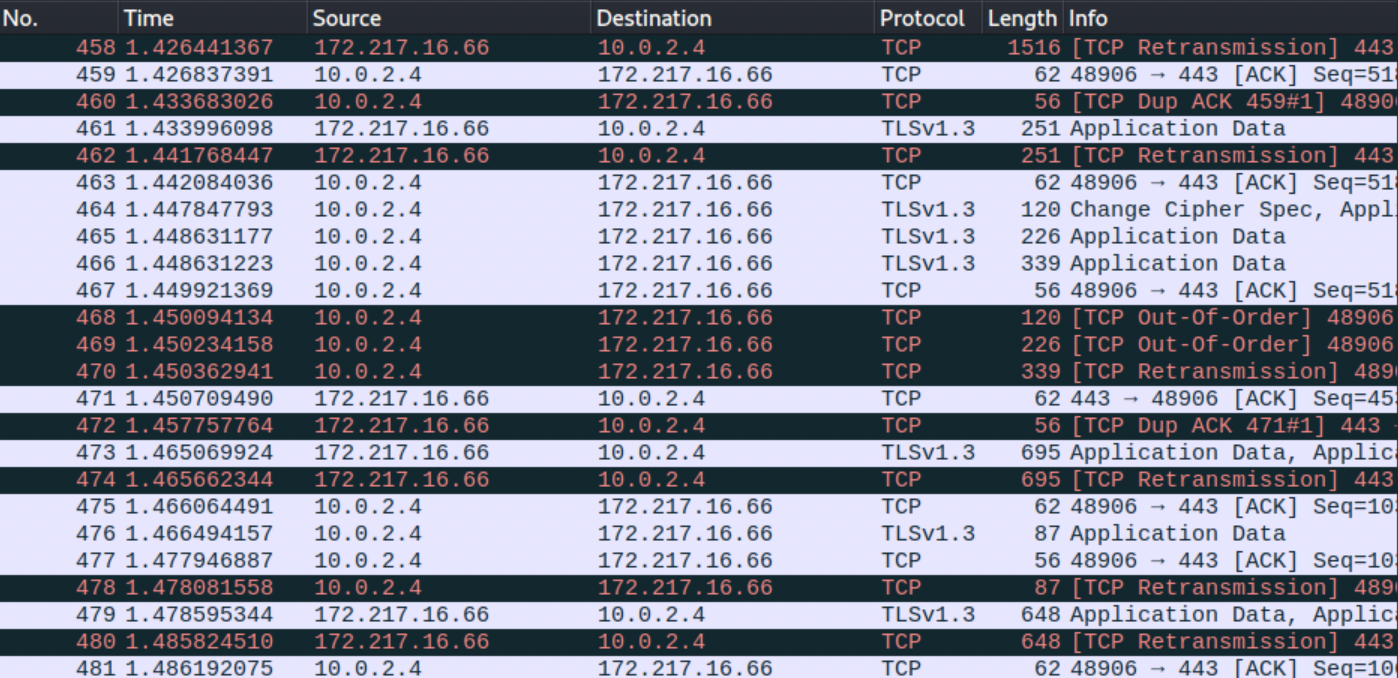
\includegraphics[width=\linewidth]{img/ws_no_vpn.png}
    \caption{Mitschnitt des Datenverkehrs bei einem \ac{MitM}}
    \label{fig:ws_mitm}
\end{figure}
\pagebreak
\section{Verschleierung des Datenverkehrs}

Nun gilt es herauszufinden, wie sich gegen eine \ac{MitM} Attacke zu schützen ist – bzw. wie der Datenverkehr verschleiert werden kann. 
Die wohl bekannteste Möglichkeit seinen Datenverkehr Dritten gegenüber zu verschleiern stellen \ac{VPN}s dar. Diese stellen eine Verbindung – auch oft als Tunnel dargestellt – zu einem Server her, welcher als eine Art Proxy die Destination der Nachrichten verschleiert. Nicht nur wird bei einem VPN die Destination verschleiert, es werden auch gesonderte Formen der Verschlüsselung angewandt, um es Angreifern schwieriger zu machen abgefangene Nachrichten zu entschlüsseln.\\ 
Dies lässt sich auf der Abbildung \ref{fig:ws_mitm_vpn} erkennen. Das VPN, welches für diese Demonstration genutzt wurde, benutzt das IAX2 Protokoll, um die Nachrichten zu übermitteln. Zudem wird dem Angreifer eine andere IP-Adresse als Destination angezeigt, obwohl das Opfer die gleiche Webseite aufruft. 

\begin{figure}
    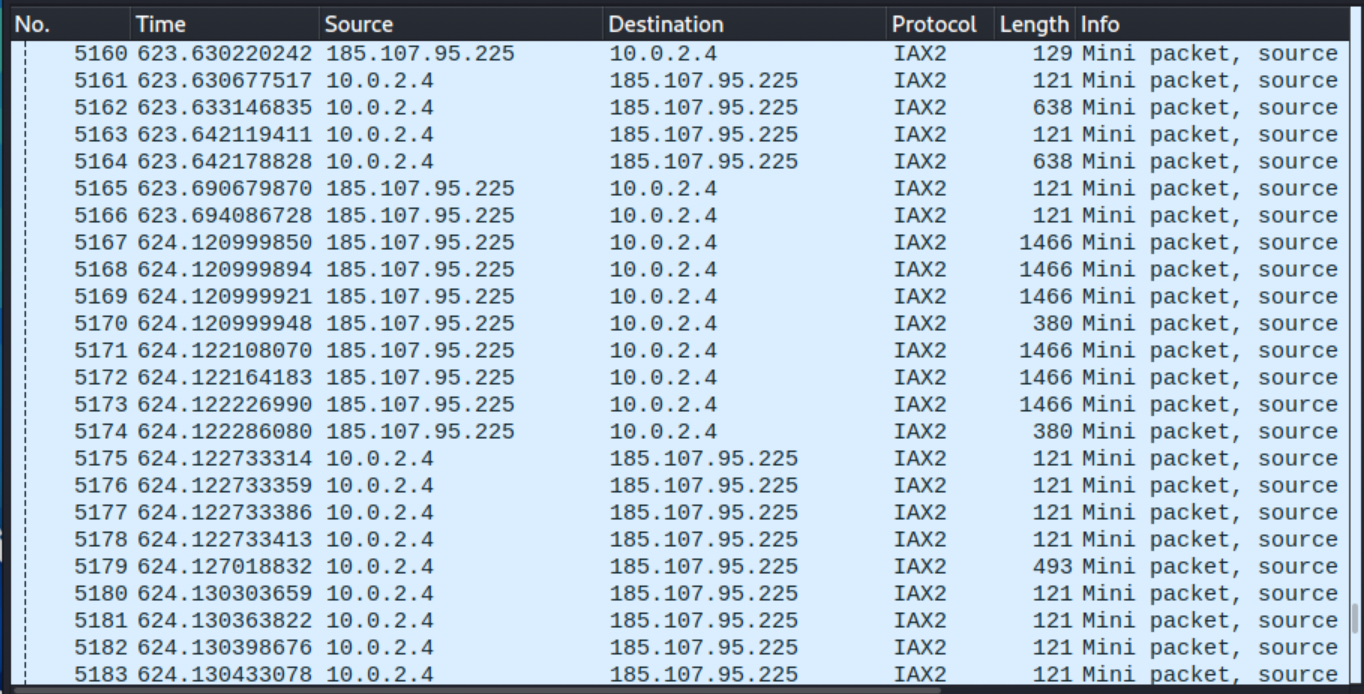
\includegraphics[width=\linewidth]{img/ws_vpn.png}
    \caption{Abgefangener Datenverkehr, welcher mittels VPN verschleiert wurde}
    \label{fig:ws_mitm_vpn}
\end{figure}
\begin{figure}
    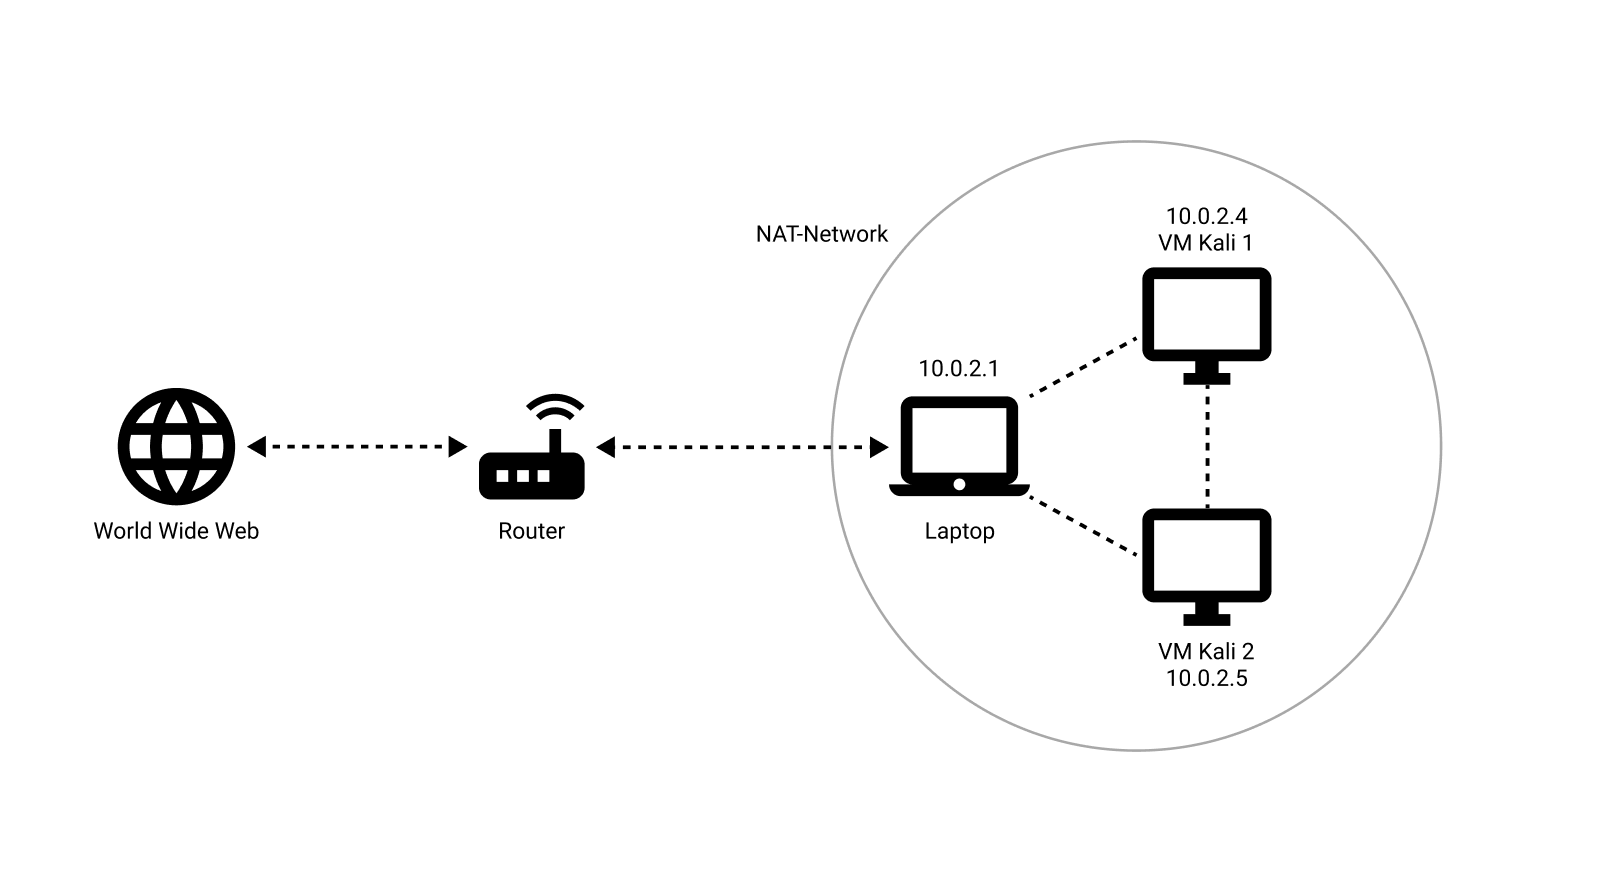
\includegraphics[width=\linewidth]{img/network_fig.png}
    \caption{Aufbau des Netzwerks}
    \label{fig:network}
\end{figure}
